\documentclass{article}
\usepackage[utf8]{inputenc}
\usepackage{hyperref}
\usepackage{graphicx}

\title{COMP140 Controller Proposal}
\author{Christopher Robertson}
\date{February 2020}

\begin{document}

\maketitle
\newpage

\section{Project Game Design}

The game design for the controller is a game where you control three sets of colours which are you able to change the hue of using a set of dials - or for debugging two keys on the keyboard. Each colour you control has a lane of queued up colours which the player must match their colour to the next colour in the lane. When the colours are matched they are able to press the dial - or a third keyboard button for debugging - to submit. The game will then either add points, or deduct lives if successful or not. As time goes on the speed of the game will increase much like any re-playable arcade game like this.

\begin{figure}[ht]
  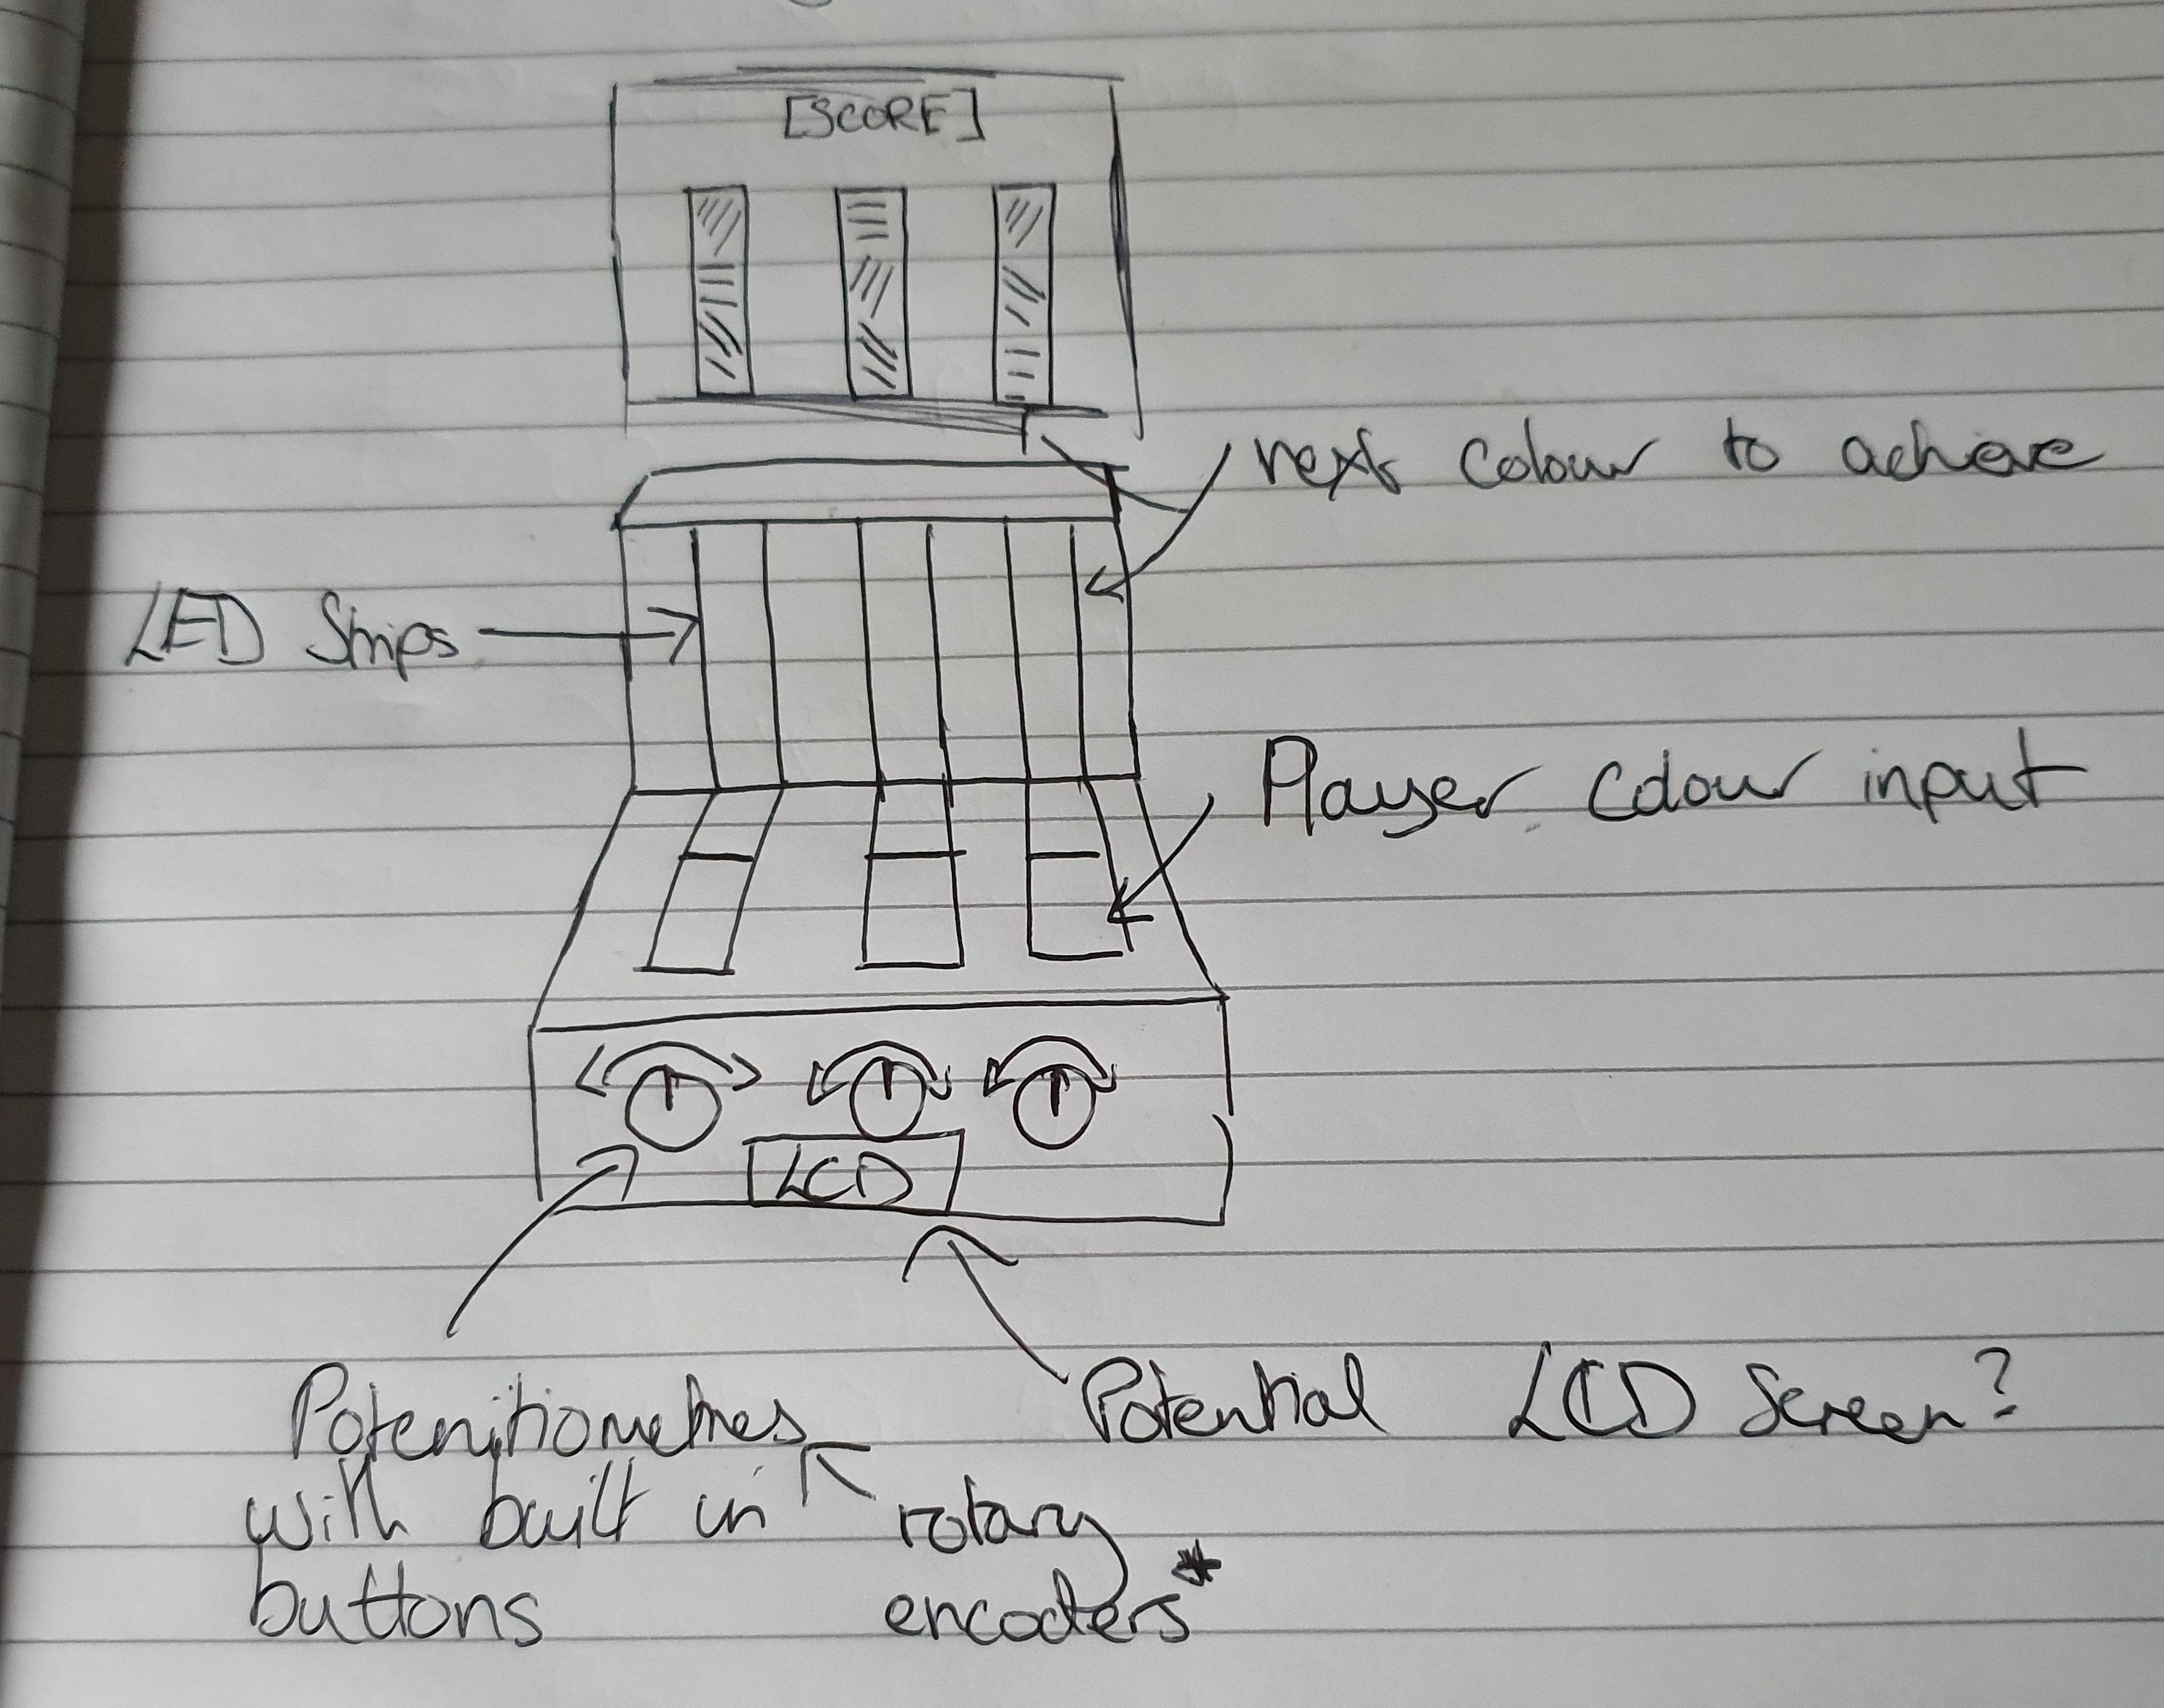
\includegraphics[width=\textwidth,height=\textheight,keepaspectratio]{controller_concept.jpg}
  \caption{Concept Art}
  \label{fig:Concept}
\end{figure}

\section{Controller Design}

I intend for the controller to be completely function by itself without the use of a screen as a sort of built in controller since it will display all of the elements using RGB LED strips. It will also display the score using either an LCD screen, or a 7 Segment Display. You are then able to control the three lane inputs with rotary encoders and submit by pressing the rotary encoders. Although you can play it by itself I do intend on making a Unity game to go along side it which will act as an extender to see the colours further down as well as other diagnostics and general gameplay.

\section{Key Components}

\begin{itemize}
    \item Rotary Encoders x 3
    \item RGB LED Strip 5m x 1
    \item LCD Screen x 1
\end{itemize}

\section{Key User Stories}

One of the main users stories would be "As a player I want to get the correct colour to gain more score" since it is the primary objective of the game for the player.

\section{Research}

\begin{figure}[ht]
  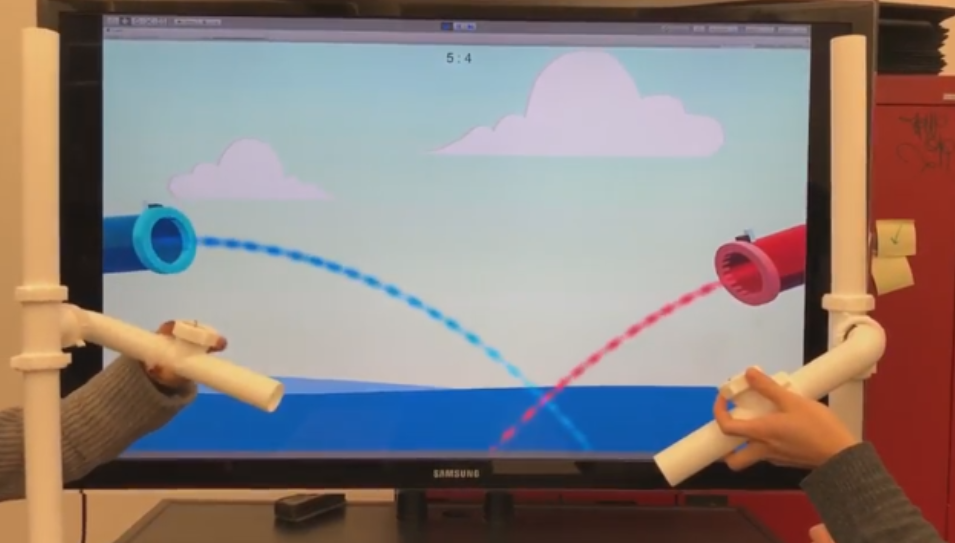
\includegraphics[width=\textwidth,height=\textheight,keepaspectratio]{lemonade.PNG}
  \caption{http://shakethatbutton.com/lemonade/}
  \label{fig:Lemonade}
\end{figure}

\subsection{Lemonade}

The first alternative controller I've found is a game named 'Lemonade' (\ref{fig:Lemonade}) which is a local coop game where two players controller two water pipes which you are able to rotate to aim the water in the game. There is also a valve on each of the pipes too which increases the pressure of the water too. The objective is to hit the lemons falling down and miss the muffins. I found this quite interesting since there is a lot of interactivity from the player since they are required to actually aim the object in the game rather than a conventional controller where a joystick would just be utilised instead.

\begin{figure}[ht]
  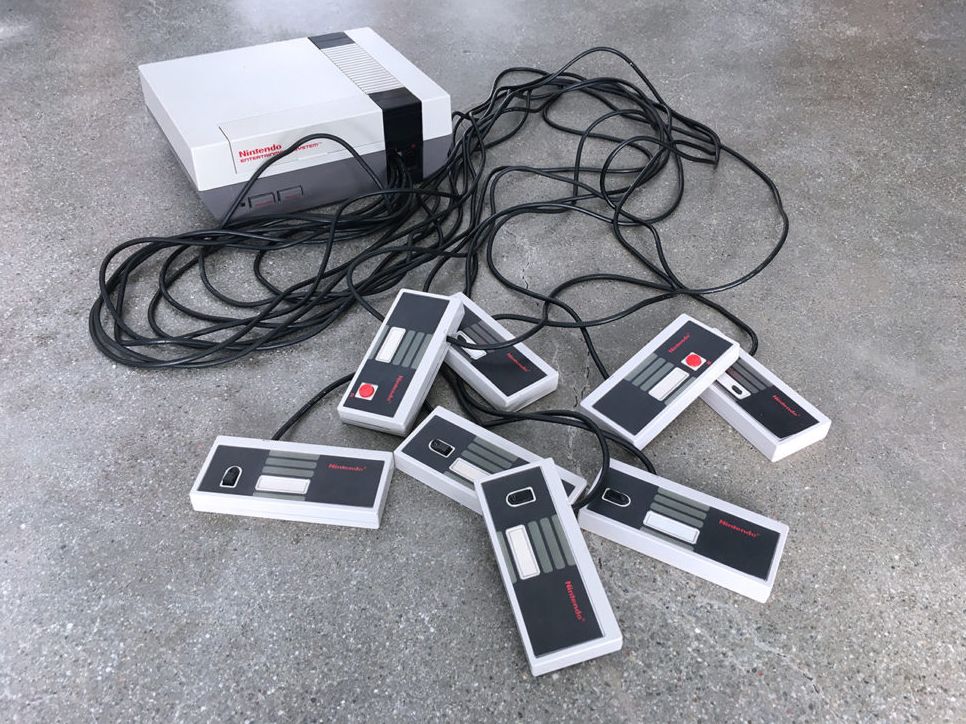
\includegraphics[width=\textwidth,height=\textheight,keepaspectratio]{ocotopad.PNG}
  \caption{http://shakethatbutton.com/the-octopad/}
  \label{fig:Octopad}
\end{figure}

\subsection{The Octopad}

Another alternative controller is the Octopad (\ref{fig:Octopad}) which is an NES system that instead of having one controller with all the buttons it has eight controllers which one button on each that in total make up an the entire control scheme of one controller. With all of these eight controllers you're able to play any NES game due to the integration. I found this quite interesting since they made a controller designed for already existing games that in theory would work with any which I quite like the idea of overall since it makes the alt-controller incredible adaptable.

\begin{figure}[ht]
  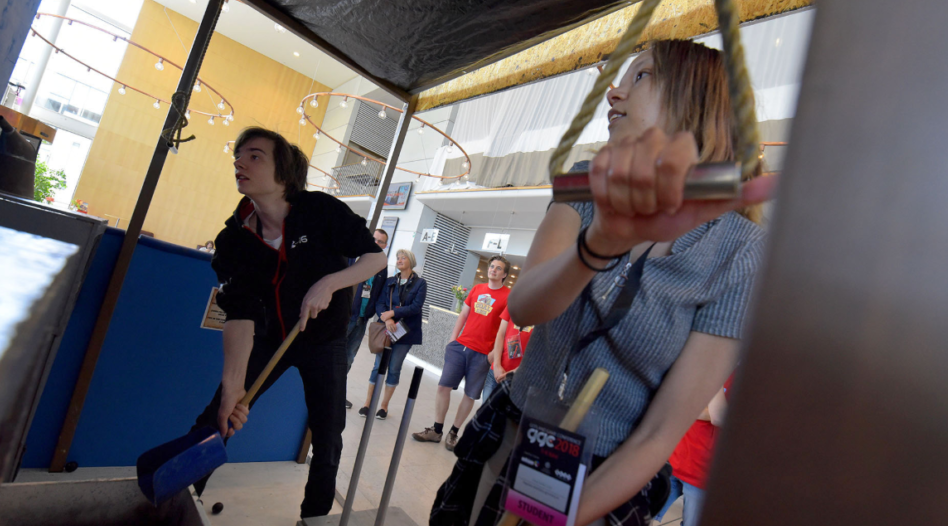
\includegraphics[width=\textwidth,height=\textheight,keepaspectratio]{coal_rush.PNG}
  \caption{http://shakethatbutton.com/coal-rush/}
  \label{fig:Coal Rush}
\end{figure}

\subsection{Coal Rush}

One alternative controller I have found is for a game called 'Coal Rush' (\ref{fig:Coal Rush}). The way you control it is through using the shovels to place coal in the furnace to increase the speed of the train and also a level to change the track that you are on to avoid obstacles. It is also a two player local co-op experience where you aim to beat the other player by being higher up on the screen. I found this one quite interesting since I really like the idea of you being able to really immersed in the experience as if you were actually controlling a locomotive train.

\end{document}
